\documentclass[11pt]{article}

    \usepackage[breakable]{tcolorbox}
    \usepackage{parskip} % Stop auto-indenting (to mimic markdown behaviour)
    
    \usepackage{iftex}
    \ifPDFTeX
    	\usepackage[T1]{fontenc}
    	\usepackage{mathpazo}
    \else
    	\usepackage{fontspec}
    \fi

    % Basic figure setup, for now with no caption control since it's done
    % automatically by Pandoc (which extracts ![](path) syntax from Markdown).
    \usepackage{graphicx}
    % Maintain compatibility with old templates. Remove in nbconvert 6.0
    \let\Oldincludegraphics\includegraphics
    % Ensure that by default, figures have no caption (until we provide a
    % proper Figure object with a Caption API and a way to capture that
    % in the conversion process - todo).
    \usepackage{caption}
    \DeclareCaptionFormat{nocaption}{}
    \captionsetup{format=nocaption,aboveskip=0pt,belowskip=0pt}

    \usepackage{float}
    \floatplacement{figure}{H} % forces figures to be placed at the correct location
    \usepackage{xcolor} % Allow colors to be defined
    \usepackage{enumerate} % Needed for markdown enumerations to work
    \usepackage{geometry} % Used to adjust the document margins
    \usepackage{amsmath} % Equations
    \usepackage{amssymb} % Equations
    \usepackage{textcomp} % defines textquotesingle
    % Hack from http://tex.stackexchange.com/a/47451/13684:
    \AtBeginDocument{%
        \def\PYZsq{\textquotesingle}% Upright quotes in Pygmentized code
    }
    \usepackage{upquote} % Upright quotes for verbatim code
    \usepackage{eurosym} % defines \euro
    \usepackage[mathletters]{ucs} % Extended unicode (utf-8) support
    \usepackage{fancyvrb} % verbatim replacement that allows latex
    \usepackage{grffile} % extends the file name processing of package graphics 
                         % to support a larger range
    \makeatletter % fix for old versions of grffile with XeLaTeX
    \@ifpackagelater{grffile}{2019/11/01}
    {
      % Do nothing on new versions
    }
    {
      \def\Gread@@xetex#1{%
        \IfFileExists{"\Gin@base".bb}%
        {\Gread@eps{\Gin@base.bb}}%
        {\Gread@@xetex@aux#1}%
      }
    }
    \makeatother
    \usepackage[Export]{adjustbox} % Used to constrain images to a maximum size
    \adjustboxset{max size={0.9\linewidth}{0.9\paperheight}}

    % The hyperref package gives us a pdf with properly built
    % internal navigation ('pdf bookmarks' for the table of contents,
    % internal cross-reference links, web links for URLs, etc.)
    \usepackage{hyperref}
    % The default LaTeX title has an obnoxious amount of whitespace. By default,
    % titling removes some of it. It also provides customization options.
    \usepackage{titling}
    \usepackage{longtable} % longtable support required by pandoc >1.10
    \usepackage{booktabs}  % table support for pandoc > 1.12.2
    \usepackage[inline]{enumitem} % IRkernel/repr support (it uses the enumerate* environment)
    \usepackage[normalem]{ulem} % ulem is needed to support strikethroughs (\sout)
                                % normalem makes italics be italics, not underlines
    \usepackage{mathrsfs}
    

    
    % Colors for the hyperref package
    \definecolor{urlcolor}{rgb}{0,.145,.698}
    \definecolor{linkcolor}{rgb}{.71,0.21,0.01}
    \definecolor{citecolor}{rgb}{.12,.54,.11}

    % ANSI colors
    \definecolor{ansi-black}{HTML}{3E424D}
    \definecolor{ansi-black-intense}{HTML}{282C36}
    \definecolor{ansi-red}{HTML}{E75C58}
    \definecolor{ansi-red-intense}{HTML}{B22B31}
    \definecolor{ansi-green}{HTML}{00A250}
    \definecolor{ansi-green-intense}{HTML}{007427}
    \definecolor{ansi-yellow}{HTML}{DDB62B}
    \definecolor{ansi-yellow-intense}{HTML}{B27D12}
    \definecolor{ansi-blue}{HTML}{208FFB}
    \definecolor{ansi-blue-intense}{HTML}{0065CA}
    \definecolor{ansi-magenta}{HTML}{D160C4}
    \definecolor{ansi-magenta-intense}{HTML}{A03196}
    \definecolor{ansi-cyan}{HTML}{60C6C8}
    \definecolor{ansi-cyan-intense}{HTML}{258F8F}
    \definecolor{ansi-white}{HTML}{C5C1B4}
    \definecolor{ansi-white-intense}{HTML}{A1A6B2}
    \definecolor{ansi-default-inverse-fg}{HTML}{FFFFFF}
    \definecolor{ansi-default-inverse-bg}{HTML}{000000}

    % common color for the border for error outputs.
    \definecolor{outerrorbackground}{HTML}{FFDFDF}

    % commands and environments needed by pandoc snippets
    % extracted from the output of `pandoc -s`
    \providecommand{\tightlist}{%
      \setlength{\itemsep}{0pt}\setlength{\parskip}{0pt}}
    \DefineVerbatimEnvironment{Highlighting}{Verbatim}{commandchars=\\\{\}}
    % Add ',fontsize=\small' for more characters per line
    \newenvironment{Shaded}{}{}
    \newcommand{\KeywordTok}[1]{\textcolor[rgb]{0.00,0.44,0.13}{\textbf{{#1}}}}
    \newcommand{\DataTypeTok}[1]{\textcolor[rgb]{0.56,0.13,0.00}{{#1}}}
    \newcommand{\DecValTok}[1]{\textcolor[rgb]{0.25,0.63,0.44}{{#1}}}
    \newcommand{\BaseNTok}[1]{\textcolor[rgb]{0.25,0.63,0.44}{{#1}}}
    \newcommand{\FloatTok}[1]{\textcolor[rgb]{0.25,0.63,0.44}{{#1}}}
    \newcommand{\CharTok}[1]{\textcolor[rgb]{0.25,0.44,0.63}{{#1}}}
    \newcommand{\StringTok}[1]{\textcolor[rgb]{0.25,0.44,0.63}{{#1}}}
    \newcommand{\CommentTok}[1]{\textcolor[rgb]{0.38,0.63,0.69}{\textit{{#1}}}}
    \newcommand{\OtherTok}[1]{\textcolor[rgb]{0.00,0.44,0.13}{{#1}}}
    \newcommand{\AlertTok}[1]{\textcolor[rgb]{1.00,0.00,0.00}{\textbf{{#1}}}}
    \newcommand{\FunctionTok}[1]{\textcolor[rgb]{0.02,0.16,0.49}{{#1}}}
    \newcommand{\RegionMarkerTok}[1]{{#1}}
    \newcommand{\ErrorTok}[1]{\textcolor[rgb]{1.00,0.00,0.00}{\textbf{{#1}}}}
    \newcommand{\NormalTok}[1]{{#1}}
    
    % Additional commands for more recent versions of Pandoc
    \newcommand{\ConstantTok}[1]{\textcolor[rgb]{0.53,0.00,0.00}{{#1}}}
    \newcommand{\SpecialCharTok}[1]{\textcolor[rgb]{0.25,0.44,0.63}{{#1}}}
    \newcommand{\VerbatimStringTok}[1]{\textcolor[rgb]{0.25,0.44,0.63}{{#1}}}
    \newcommand{\SpecialStringTok}[1]{\textcolor[rgb]{0.73,0.40,0.53}{{#1}}}
    \newcommand{\ImportTok}[1]{{#1}}
    \newcommand{\DocumentationTok}[1]{\textcolor[rgb]{0.73,0.13,0.13}{\textit{{#1}}}}
    \newcommand{\AnnotationTok}[1]{\textcolor[rgb]{0.38,0.63,0.69}{\textbf{\textit{{#1}}}}}
    \newcommand{\CommentVarTok}[1]{\textcolor[rgb]{0.38,0.63,0.69}{\textbf{\textit{{#1}}}}}
    \newcommand{\VariableTok}[1]{\textcolor[rgb]{0.10,0.09,0.49}{{#1}}}
    \newcommand{\ControlFlowTok}[1]{\textcolor[rgb]{0.00,0.44,0.13}{\textbf{{#1}}}}
    \newcommand{\OperatorTok}[1]{\textcolor[rgb]{0.40,0.40,0.40}{{#1}}}
    \newcommand{\BuiltInTok}[1]{{#1}}
    \newcommand{\ExtensionTok}[1]{{#1}}
    \newcommand{\PreprocessorTok}[1]{\textcolor[rgb]{0.74,0.48,0.00}{{#1}}}
    \newcommand{\AttributeTok}[1]{\textcolor[rgb]{0.49,0.56,0.16}{{#1}}}
    \newcommand{\InformationTok}[1]{\textcolor[rgb]{0.38,0.63,0.69}{\textbf{\textit{{#1}}}}}
    \newcommand{\WarningTok}[1]{\textcolor[rgb]{0.38,0.63,0.69}{\textbf{\textit{{#1}}}}}
    
    
    % Define a nice break command that doesn't care if a line doesn't already
    % exist.
    \def\br{\hspace*{\fill} \\* }
    % Math Jax compatibility definitions
    \def\gt{>}
    \def\lt{<}
    \let\Oldtex\TeX
    \let\Oldlatex\LaTeX
    \renewcommand{\TeX}{\textrm{\Oldtex}}
    \renewcommand{\LaTeX}{\textrm{\Oldlatex}}
    % Document parameters
    % Document title
    \title{5-Localization-1-LeastSquares}
    
    
    
    
    
% Pygments definitions
\makeatletter
\def\PY@reset{\let\PY@it=\relax \let\PY@bf=\relax%
    \let\PY@ul=\relax \let\PY@tc=\relax%
    \let\PY@bc=\relax \let\PY@ff=\relax}
\def\PY@tok#1{\csname PY@tok@#1\endcsname}
\def\PY@toks#1+{\ifx\relax#1\empty\else%
    \PY@tok{#1}\expandafter\PY@toks\fi}
\def\PY@do#1{\PY@bc{\PY@tc{\PY@ul{%
    \PY@it{\PY@bf{\PY@ff{#1}}}}}}}
\def\PY#1#2{\PY@reset\PY@toks#1+\relax+\PY@do{#2}}

\expandafter\def\csname PY@tok@w\endcsname{\def\PY@tc##1{\textcolor[rgb]{0.73,0.73,0.73}{##1}}}
\expandafter\def\csname PY@tok@c\endcsname{\let\PY@it=\textit\def\PY@tc##1{\textcolor[rgb]{0.25,0.50,0.50}{##1}}}
\expandafter\def\csname PY@tok@cp\endcsname{\def\PY@tc##1{\textcolor[rgb]{0.74,0.48,0.00}{##1}}}
\expandafter\def\csname PY@tok@k\endcsname{\let\PY@bf=\textbf\def\PY@tc##1{\textcolor[rgb]{0.00,0.50,0.00}{##1}}}
\expandafter\def\csname PY@tok@kp\endcsname{\def\PY@tc##1{\textcolor[rgb]{0.00,0.50,0.00}{##1}}}
\expandafter\def\csname PY@tok@kt\endcsname{\def\PY@tc##1{\textcolor[rgb]{0.69,0.00,0.25}{##1}}}
\expandafter\def\csname PY@tok@o\endcsname{\def\PY@tc##1{\textcolor[rgb]{0.40,0.40,0.40}{##1}}}
\expandafter\def\csname PY@tok@ow\endcsname{\let\PY@bf=\textbf\def\PY@tc##1{\textcolor[rgb]{0.67,0.13,1.00}{##1}}}
\expandafter\def\csname PY@tok@nb\endcsname{\def\PY@tc##1{\textcolor[rgb]{0.00,0.50,0.00}{##1}}}
\expandafter\def\csname PY@tok@nf\endcsname{\def\PY@tc##1{\textcolor[rgb]{0.00,0.00,1.00}{##1}}}
\expandafter\def\csname PY@tok@nc\endcsname{\let\PY@bf=\textbf\def\PY@tc##1{\textcolor[rgb]{0.00,0.00,1.00}{##1}}}
\expandafter\def\csname PY@tok@nn\endcsname{\let\PY@bf=\textbf\def\PY@tc##1{\textcolor[rgb]{0.00,0.00,1.00}{##1}}}
\expandafter\def\csname PY@tok@ne\endcsname{\let\PY@bf=\textbf\def\PY@tc##1{\textcolor[rgb]{0.82,0.25,0.23}{##1}}}
\expandafter\def\csname PY@tok@nv\endcsname{\def\PY@tc##1{\textcolor[rgb]{0.10,0.09,0.49}{##1}}}
\expandafter\def\csname PY@tok@no\endcsname{\def\PY@tc##1{\textcolor[rgb]{0.53,0.00,0.00}{##1}}}
\expandafter\def\csname PY@tok@nl\endcsname{\def\PY@tc##1{\textcolor[rgb]{0.63,0.63,0.00}{##1}}}
\expandafter\def\csname PY@tok@ni\endcsname{\let\PY@bf=\textbf\def\PY@tc##1{\textcolor[rgb]{0.60,0.60,0.60}{##1}}}
\expandafter\def\csname PY@tok@na\endcsname{\def\PY@tc##1{\textcolor[rgb]{0.49,0.56,0.16}{##1}}}
\expandafter\def\csname PY@tok@nt\endcsname{\let\PY@bf=\textbf\def\PY@tc##1{\textcolor[rgb]{0.00,0.50,0.00}{##1}}}
\expandafter\def\csname PY@tok@nd\endcsname{\def\PY@tc##1{\textcolor[rgb]{0.67,0.13,1.00}{##1}}}
\expandafter\def\csname PY@tok@s\endcsname{\def\PY@tc##1{\textcolor[rgb]{0.73,0.13,0.13}{##1}}}
\expandafter\def\csname PY@tok@sd\endcsname{\let\PY@it=\textit\def\PY@tc##1{\textcolor[rgb]{0.73,0.13,0.13}{##1}}}
\expandafter\def\csname PY@tok@si\endcsname{\let\PY@bf=\textbf\def\PY@tc##1{\textcolor[rgb]{0.73,0.40,0.53}{##1}}}
\expandafter\def\csname PY@tok@se\endcsname{\let\PY@bf=\textbf\def\PY@tc##1{\textcolor[rgb]{0.73,0.40,0.13}{##1}}}
\expandafter\def\csname PY@tok@sr\endcsname{\def\PY@tc##1{\textcolor[rgb]{0.73,0.40,0.53}{##1}}}
\expandafter\def\csname PY@tok@ss\endcsname{\def\PY@tc##1{\textcolor[rgb]{0.10,0.09,0.49}{##1}}}
\expandafter\def\csname PY@tok@sx\endcsname{\def\PY@tc##1{\textcolor[rgb]{0.00,0.50,0.00}{##1}}}
\expandafter\def\csname PY@tok@m\endcsname{\def\PY@tc##1{\textcolor[rgb]{0.40,0.40,0.40}{##1}}}
\expandafter\def\csname PY@tok@gh\endcsname{\let\PY@bf=\textbf\def\PY@tc##1{\textcolor[rgb]{0.00,0.00,0.50}{##1}}}
\expandafter\def\csname PY@tok@gu\endcsname{\let\PY@bf=\textbf\def\PY@tc##1{\textcolor[rgb]{0.50,0.00,0.50}{##1}}}
\expandafter\def\csname PY@tok@gd\endcsname{\def\PY@tc##1{\textcolor[rgb]{0.63,0.00,0.00}{##1}}}
\expandafter\def\csname PY@tok@gi\endcsname{\def\PY@tc##1{\textcolor[rgb]{0.00,0.63,0.00}{##1}}}
\expandafter\def\csname PY@tok@gr\endcsname{\def\PY@tc##1{\textcolor[rgb]{1.00,0.00,0.00}{##1}}}
\expandafter\def\csname PY@tok@ge\endcsname{\let\PY@it=\textit}
\expandafter\def\csname PY@tok@gs\endcsname{\let\PY@bf=\textbf}
\expandafter\def\csname PY@tok@gp\endcsname{\let\PY@bf=\textbf\def\PY@tc##1{\textcolor[rgb]{0.00,0.00,0.50}{##1}}}
\expandafter\def\csname PY@tok@go\endcsname{\def\PY@tc##1{\textcolor[rgb]{0.53,0.53,0.53}{##1}}}
\expandafter\def\csname PY@tok@gt\endcsname{\def\PY@tc##1{\textcolor[rgb]{0.00,0.27,0.87}{##1}}}
\expandafter\def\csname PY@tok@err\endcsname{\def\PY@bc##1{\setlength{\fboxsep}{0pt}\fcolorbox[rgb]{1.00,0.00,0.00}{1,1,1}{\strut ##1}}}
\expandafter\def\csname PY@tok@kc\endcsname{\let\PY@bf=\textbf\def\PY@tc##1{\textcolor[rgb]{0.00,0.50,0.00}{##1}}}
\expandafter\def\csname PY@tok@kd\endcsname{\let\PY@bf=\textbf\def\PY@tc##1{\textcolor[rgb]{0.00,0.50,0.00}{##1}}}
\expandafter\def\csname PY@tok@kn\endcsname{\let\PY@bf=\textbf\def\PY@tc##1{\textcolor[rgb]{0.00,0.50,0.00}{##1}}}
\expandafter\def\csname PY@tok@kr\endcsname{\let\PY@bf=\textbf\def\PY@tc##1{\textcolor[rgb]{0.00,0.50,0.00}{##1}}}
\expandafter\def\csname PY@tok@bp\endcsname{\def\PY@tc##1{\textcolor[rgb]{0.00,0.50,0.00}{##1}}}
\expandafter\def\csname PY@tok@fm\endcsname{\def\PY@tc##1{\textcolor[rgb]{0.00,0.00,1.00}{##1}}}
\expandafter\def\csname PY@tok@vc\endcsname{\def\PY@tc##1{\textcolor[rgb]{0.10,0.09,0.49}{##1}}}
\expandafter\def\csname PY@tok@vg\endcsname{\def\PY@tc##1{\textcolor[rgb]{0.10,0.09,0.49}{##1}}}
\expandafter\def\csname PY@tok@vi\endcsname{\def\PY@tc##1{\textcolor[rgb]{0.10,0.09,0.49}{##1}}}
\expandafter\def\csname PY@tok@vm\endcsname{\def\PY@tc##1{\textcolor[rgb]{0.10,0.09,0.49}{##1}}}
\expandafter\def\csname PY@tok@sa\endcsname{\def\PY@tc##1{\textcolor[rgb]{0.73,0.13,0.13}{##1}}}
\expandafter\def\csname PY@tok@sb\endcsname{\def\PY@tc##1{\textcolor[rgb]{0.73,0.13,0.13}{##1}}}
\expandafter\def\csname PY@tok@sc\endcsname{\def\PY@tc##1{\textcolor[rgb]{0.73,0.13,0.13}{##1}}}
\expandafter\def\csname PY@tok@dl\endcsname{\def\PY@tc##1{\textcolor[rgb]{0.73,0.13,0.13}{##1}}}
\expandafter\def\csname PY@tok@s2\endcsname{\def\PY@tc##1{\textcolor[rgb]{0.73,0.13,0.13}{##1}}}
\expandafter\def\csname PY@tok@sh\endcsname{\def\PY@tc##1{\textcolor[rgb]{0.73,0.13,0.13}{##1}}}
\expandafter\def\csname PY@tok@s1\endcsname{\def\PY@tc##1{\textcolor[rgb]{0.73,0.13,0.13}{##1}}}
\expandafter\def\csname PY@tok@mb\endcsname{\def\PY@tc##1{\textcolor[rgb]{0.40,0.40,0.40}{##1}}}
\expandafter\def\csname PY@tok@mf\endcsname{\def\PY@tc##1{\textcolor[rgb]{0.40,0.40,0.40}{##1}}}
\expandafter\def\csname PY@tok@mh\endcsname{\def\PY@tc##1{\textcolor[rgb]{0.40,0.40,0.40}{##1}}}
\expandafter\def\csname PY@tok@mi\endcsname{\def\PY@tc##1{\textcolor[rgb]{0.40,0.40,0.40}{##1}}}
\expandafter\def\csname PY@tok@il\endcsname{\def\PY@tc##1{\textcolor[rgb]{0.40,0.40,0.40}{##1}}}
\expandafter\def\csname PY@tok@mo\endcsname{\def\PY@tc##1{\textcolor[rgb]{0.40,0.40,0.40}{##1}}}
\expandafter\def\csname PY@tok@ch\endcsname{\let\PY@it=\textit\def\PY@tc##1{\textcolor[rgb]{0.25,0.50,0.50}{##1}}}
\expandafter\def\csname PY@tok@cm\endcsname{\let\PY@it=\textit\def\PY@tc##1{\textcolor[rgb]{0.25,0.50,0.50}{##1}}}
\expandafter\def\csname PY@tok@cpf\endcsname{\let\PY@it=\textit\def\PY@tc##1{\textcolor[rgb]{0.25,0.50,0.50}{##1}}}
\expandafter\def\csname PY@tok@c1\endcsname{\let\PY@it=\textit\def\PY@tc##1{\textcolor[rgb]{0.25,0.50,0.50}{##1}}}
\expandafter\def\csname PY@tok@cs\endcsname{\let\PY@it=\textit\def\PY@tc##1{\textcolor[rgb]{0.25,0.50,0.50}{##1}}}

\def\PYZbs{\char`\\}
\def\PYZus{\char`\_}
\def\PYZob{\char`\{}
\def\PYZcb{\char`\}}
\def\PYZca{\char`\^}
\def\PYZam{\char`\&}
\def\PYZlt{\char`\<}
\def\PYZgt{\char`\>}
\def\PYZsh{\char`\#}
\def\PYZpc{\char`\%}
\def\PYZdl{\char`\$}
\def\PYZhy{\char`\-}
\def\PYZsq{\char`\'}
\def\PYZdq{\char`\"}
\def\PYZti{\char`\~}
% for compatibility with earlier versions
\def\PYZat{@}
\def\PYZlb{[}
\def\PYZrb{]}
\makeatother


    % For linebreaks inside Verbatim environment from package fancyvrb. 
    \makeatletter
        \newbox\Wrappedcontinuationbox 
        \newbox\Wrappedvisiblespacebox 
        \newcommand*\Wrappedvisiblespace {\textcolor{red}{\textvisiblespace}} 
        \newcommand*\Wrappedcontinuationsymbol {\textcolor{red}{\llap{\tiny$\m@th\hookrightarrow$}}} 
        \newcommand*\Wrappedcontinuationindent {3ex } 
        \newcommand*\Wrappedafterbreak {\kern\Wrappedcontinuationindent\copy\Wrappedcontinuationbox} 
        % Take advantage of the already applied Pygments mark-up to insert 
        % potential linebreaks for TeX processing. 
        %        {, <, #, %, $, ' and ": go to next line. 
        %        _, }, ^, &, >, - and ~: stay at end of broken line. 
        % Use of \textquotesingle for straight quote. 
        \newcommand*\Wrappedbreaksatspecials {% 
            \def\PYGZus{\discretionary{\char`\_}{\Wrappedafterbreak}{\char`\_}}% 
            \def\PYGZob{\discretionary{}{\Wrappedafterbreak\char`\{}{\char`\{}}% 
            \def\PYGZcb{\discretionary{\char`\}}{\Wrappedafterbreak}{\char`\}}}% 
            \def\PYGZca{\discretionary{\char`\^}{\Wrappedafterbreak}{\char`\^}}% 
            \def\PYGZam{\discretionary{\char`\&}{\Wrappedafterbreak}{\char`\&}}% 
            \def\PYGZlt{\discretionary{}{\Wrappedafterbreak\char`\<}{\char`\<}}% 
            \def\PYGZgt{\discretionary{\char`\>}{\Wrappedafterbreak}{\char`\>}}% 
            \def\PYGZsh{\discretionary{}{\Wrappedafterbreak\char`\#}{\char`\#}}% 
            \def\PYGZpc{\discretionary{}{\Wrappedafterbreak\char`\%}{\char`\%}}% 
            \def\PYGZdl{\discretionary{}{\Wrappedafterbreak\char`\$}{\char`\$}}% 
            \def\PYGZhy{\discretionary{\char`\-}{\Wrappedafterbreak}{\char`\-}}% 
            \def\PYGZsq{\discretionary{}{\Wrappedafterbreak\textquotesingle}{\textquotesingle}}% 
            \def\PYGZdq{\discretionary{}{\Wrappedafterbreak\char`\"}{\char`\"}}% 
            \def\PYGZti{\discretionary{\char`\~}{\Wrappedafterbreak}{\char`\~}}% 
        } 
        % Some characters . , ; ? ! / are not pygmentized. 
        % This macro makes them "active" and they will insert potential linebreaks 
        \newcommand*\Wrappedbreaksatpunct {% 
            \lccode`\~`\.\lowercase{\def~}{\discretionary{\hbox{\char`\.}}{\Wrappedafterbreak}{\hbox{\char`\.}}}% 
            \lccode`\~`\,\lowercase{\def~}{\discretionary{\hbox{\char`\,}}{\Wrappedafterbreak}{\hbox{\char`\,}}}% 
            \lccode`\~`\;\lowercase{\def~}{\discretionary{\hbox{\char`\;}}{\Wrappedafterbreak}{\hbox{\char`\;}}}% 
            \lccode`\~`\:\lowercase{\def~}{\discretionary{\hbox{\char`\:}}{\Wrappedafterbreak}{\hbox{\char`\:}}}% 
            \lccode`\~`\?\lowercase{\def~}{\discretionary{\hbox{\char`\?}}{\Wrappedafterbreak}{\hbox{\char`\?}}}% 
            \lccode`\~`\!\lowercase{\def~}{\discretionary{\hbox{\char`\!}}{\Wrappedafterbreak}{\hbox{\char`\!}}}% 
            \lccode`\~`\/\lowercase{\def~}{\discretionary{\hbox{\char`\/}}{\Wrappedafterbreak}{\hbox{\char`\/}}}% 
            \catcode`\.\active
            \catcode`\,\active 
            \catcode`\;\active
            \catcode`\:\active
            \catcode`\?\active
            \catcode`\!\active
            \catcode`\/\active 
            \lccode`\~`\~ 	
        }
    \makeatother

    \let\OriginalVerbatim=\Verbatim
    \makeatletter
    \renewcommand{\Verbatim}[1][1]{%
        %\parskip\z@skip
        \sbox\Wrappedcontinuationbox {\Wrappedcontinuationsymbol}%
        \sbox\Wrappedvisiblespacebox {\FV@SetupFont\Wrappedvisiblespace}%
        \def\FancyVerbFormatLine ##1{\hsize\linewidth
            \vtop{\raggedright\hyphenpenalty\z@\exhyphenpenalty\z@
                \doublehyphendemerits\z@\finalhyphendemerits\z@
                \strut ##1\strut}%
        }%
        % If the linebreak is at a space, the latter will be displayed as visible
        % space at end of first line, and a continuation symbol starts next line.
        % Stretch/shrink are however usually zero for typewriter font.
        \def\FV@Space {%
            \nobreak\hskip\z@ plus\fontdimen3\font minus\fontdimen4\font
            \discretionary{\copy\Wrappedvisiblespacebox}{\Wrappedafterbreak}
            {\kern\fontdimen2\font}%
        }%
        
        % Allow breaks at special characters using \PYG... macros.
        \Wrappedbreaksatspecials
        % Breaks at punctuation characters . , ; ? ! and / need catcode=\active 	
        \OriginalVerbatim[#1,codes*=\Wrappedbreaksatpunct]%
    }
    \makeatother

    % Exact colors from NB
    \definecolor{incolor}{HTML}{303F9F}
    \definecolor{outcolor}{HTML}{D84315}
    \definecolor{cellborder}{HTML}{CFCFCF}
    \definecolor{cellbackground}{HTML}{F7F7F7}
    
    % prompt
    \makeatletter
    \newcommand{\boxspacing}{\kern\kvtcb@left@rule\kern\kvtcb@boxsep}
    \makeatother
    \newcommand{\prompt}[4]{
        {\ttfamily\llap{{\color{#2}[#3]:\hspace{3pt}#4}}\vspace{-\baselineskip}}
    }
    

    
    % Prevent overflowing lines due to hard-to-break entities
    \sloppy 
    % Setup hyperref package
    \hypersetup{
      breaklinks=true,  % so long urls are correctly broken across lines
      colorlinks=true,
      urlcolor=urlcolor,
      linkcolor=linkcolor,
      citecolor=citecolor,
      }
    % Slightly bigger margins than the latex defaults
    
    \geometry{verbose,tmargin=1in,bmargin=1in,lmargin=1in,rmargin=1in}
    
    

\begin{document}
    
    \maketitle
    
    

    
    \hypertarget{least-squares-global-localization}{%
\section{5.1 Least Squares Global
Localization}\label{least-squares-global-localization}}

Least Squares Positioning is a well-known algorithm for estimating the
robot localization \(x\) given a set of known landmarks in a map. Least
Squares is akin to find the best pose \(\hat{x}\) by solving a system of
equations of the form:

\[z_{m \times 1} = H_{m \times n} \cdot x_{n \times 1}\]

where: - \(n\) is the length of the pose (\(n=3\) in our case, position
plus orientation), - \(m\) represents the number of observations, and -
\(H\) is the matrix that codifies the observation model relating the
measurement \(z\) with the robot pose \(x\). For example, if we are
using a pointer to measure the distance to a wall, the element
associated with each \(z\) in \(H\) takes the value 1.

This simple concept, nevertheless, has to be modified in order to be
used in real scenarios:

    \hypertarget{pseudo-inverse}{%
\subsection{5.1.1 Pseudo-inverse}\label{pseudo-inverse}}

Generally, to solve an equation system, we only need as many equations
as variables. In the robot localization problem, each observation \(z\)
sets an equation, while the variables are the components of the
state/pose, \(x\).

In such a case, where \(n=m\), a direct attempt to this problem exists:

\[x = H ^{-1} z\]

So a unique solution exists if \(H\) is invertible, that is, \(H\) is a
square matrix with \(det(H) \neq 0\).

However, in real scenarios typically there are available more
observations than variables. An approach to address this could be to
drop some of the additional equations, but given that observations \(z\)
are inaccurate (they have been affected by some noise), we may use the
additional information to try to mitigate such noise. However, by doing
that \(H\) is no a squared matrix anymore, hence not being invertible.

Two tools can help us at this point. The first one is the utilization of
\textbf{Least Squares} to find the closest possible \(\hat{x}\),
i.e.~the one where the the error (\(e = Hx -z\)) is minimal:

\[ \hat x = \arg\min_{x} e^Te = [(Hx-z)^T(Hx-z)] = \arg\min_x || h(x) -z ||^2\]

which has a close form solution using the \textbf{pseudo-inverse} of a
matrix:

\[\hat{x} = \underbrace{(H^T H)^{-1} H^T}_{\textit{pseudo-inverse }(H^+)} z\]

The \textbf{pseudo-inverse}, in contrast to the normal inverse
operation, can be used in non-square matrices!

    \begin{tcolorbox}[breakable, size=fbox, boxrule=1pt, pad at break*=1mm,colback=cellbackground, colframe=cellborder]
\prompt{In}{incolor}{1}{\boxspacing}
\begin{Verbatim}[commandchars=\\\{\}]
\PY{c+c1}{\PYZsh{}\PYZpc{}matplotlib notebook}
\PY{c+c1}{\PYZsh{}\PYZpc{}matplotlib inline}

\PY{c+c1}{\PYZsh{} IMPORTS}

\PY{k+kn}{import} \PY{n+nn}{math}

\PY{k+kn}{import} \PY{n+nn}{numpy} \PY{k}{as} \PY{n+nn}{np}
\PY{k+kn}{from} \PY{n+nn}{numpy} \PY{k+kn}{import} \PY{n}{linalg}
\PY{k+kn}{import} \PY{n+nn}{matplotlib}
\PY{n}{matplotlib}\PY{o}{.}\PY{n}{use}\PY{p}{(}\PY{l+s+s1}{\PYZsq{}}\PY{l+s+s1}{TkAgg}\PY{l+s+s1}{\PYZsq{}}\PY{p}{)}
\PY{k+kn}{import} \PY{n+nn}{matplotlib}\PY{n+nn}{.}\PY{n+nn}{pyplot} \PY{k}{as} \PY{n+nn}{plt}
\PY{k+kn}{import} \PY{n+nn}{scipy}
\PY{k+kn}{from} \PY{n+nn}{scipy} \PY{k+kn}{import} \PY{n}{stats}

\PY{k+kn}{import} \PY{n+nn}{sys}
\PY{n}{sys}\PY{o}{.}\PY{n}{path}\PY{o}{.}\PY{n}{append}\PY{p}{(}\PY{l+s+s2}{\PYZdq{}}\PY{l+s+s2}{..}\PY{l+s+s2}{\PYZdq{}}\PY{p}{)}
\PY{k+kn}{from} \PY{n+nn}{utils}\PY{n+nn}{.}\PY{n+nn}{PlotEllipse} \PY{k+kn}{import} \PY{n}{PlotEllipse}
\PY{k+kn}{from} \PY{n+nn}{utils}\PY{n+nn}{.}\PY{n+nn}{DrawRobot} \PY{k+kn}{import} \PY{n}{DrawRobot}
\PY{k+kn}{from} \PY{n+nn}{utils}\PY{n+nn}{.}\PY{n+nn}{tcomp} \PY{k+kn}{import} \PY{n}{tcomp}
\PY{k+kn}{from} \PY{n+nn}{utils}\PY{n+nn}{.}\PY{n+nn}{tinv} \PY{k+kn}{import} \PY{n}{tinv}\PY{p}{,} \PY{n}{jac\PYZus{}tinv1} \PY{k}{as} \PY{n}{jac\PYZus{}tinv}
\PY{k+kn}{from} \PY{n+nn}{utils}\PY{n+nn}{.}\PY{n+nn}{Jacobians} \PY{k+kn}{import} \PY{n}{J1}\PY{p}{,} \PY{n}{J2}
\end{Verbatim}
\end{tcolorbox}

    \hypertarget{assignment-1-playing-with-a-robot-in-a-corridor}{%
\subsubsection{\texorpdfstring{\textbf{{ASSIGNMENT 1: Playing with a
robot in a
corridor}}}{ASSIGNMENT 1: Playing with a robot in a corridor}}\label{assignment-1-playing-with-a-robot-in-a-corridor}}

The following code illustrates a simple scenario where a robot is in a
corridor looking at a door, which is placed at the origin of the
reference system (see Fig.1). The robot is equipped with a laser scanner
able to measure distances, and takes a number of observations \(z\). The
robot is placed 3 meters away from the door, but this information is
unknown for it. \textbf{Your goal is} to estimate the position of the
robot in this 1D world using such measurements. \(\\[5pt]\)

\begin{figure}
\centering
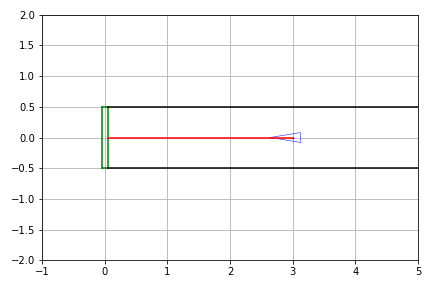
\includegraphics{images/corridor.png}
\end{figure}
Fig. 1: Simple 1D scenario with a robot equipped with a laser scanner
measuring distance to a door.

The following code cell shows the dimensions of all the actors involved
in LS-positioning. Complete it for computing the robot pose \(x\) from
the available information. \emph{Recall
\href{https://numpy.org/doc/stable/reference/generated/numpy.linalg.inv.html}{\texttt{np.linalg.inv()}}.}

    \begin{tcolorbox}[breakable, size=fbox, boxrule=1pt, pad at break*=1mm,colback=cellbackground, colframe=cellborder]
\prompt{In}{incolor}{2}{\boxspacing}
\begin{Verbatim}[commandchars=\\\{\}]
\PY{c+c1}{\PYZsh{} Set the robot pose to unknown}
\PY{n}{x} \PY{o}{=} \PY{n}{np}\PY{o}{.}\PY{n}{vstack}\PY{p}{(}\PY{n}{np}\PY{o}{.}\PY{n}{array}\PY{p}{(}\PY{p}{[}\PY{k+kc}{None}\PY{p}{]}\PY{p}{)}\PY{p}{)}

\PY{c+c1}{\PYZsh{} Sensor measurements to the door}
\PY{n}{z} \PY{o}{=} \PY{n}{np}\PY{o}{.}\PY{n}{vstack}\PY{p}{(}\PY{n}{np}\PY{o}{.}\PY{n}{array}\PY{p}{(}\PY{p}{[}\PY{l+m+mf}{3.7}\PY{p}{,}\PY{l+m+mf}{2.9}\PY{p}{,}\PY{l+m+mf}{3.6}\PY{p}{,}\PY{l+m+mf}{2.5}\PY{p}{,}\PY{l+m+mf}{3.5}\PY{p}{]}\PY{p}{)}\PY{p}{)}

\PY{c+c1}{\PYZsh{} Observation model}
\PY{n}{H} \PY{o}{=} \PY{n}{np}\PY{o}{.}\PY{n}{ones}\PY{p}{(}\PY{n}{np}\PY{o}{.}\PY{n}{array}\PY{p}{(}\PY{p}{[}\PY{l+m+mi}{5}\PY{p}{,}\PY{l+m+mi}{1}\PY{p}{]}\PY{p}{)}\PY{p}{)}

\PY{n+nb}{print} \PY{p}{(}\PY{l+s+s2}{\PYZdq{}}\PY{l+s+s2}{Dimensions:}\PY{l+s+s2}{\PYZdq{}}\PY{p}{)}
\PY{n+nb}{print} \PY{p}{(}\PY{l+s+s2}{\PYZdq{}}\PY{l+s+s2}{Pose x:         }\PY{l+s+s2}{\PYZdq{}} \PY{o}{+} \PY{n+nb}{str}\PY{p}{(}\PY{n}{x}\PY{o}{.}\PY{n}{shape}\PY{p}{)}\PY{p}{)}
\PY{n+nb}{print} \PY{p}{(}\PY{l+s+s2}{\PYZdq{}}\PY{l+s+s2}{Observations z: }\PY{l+s+s2}{\PYZdq{}} \PY{o}{+} \PY{n+nb}{str}\PY{p}{(}\PY{n}{z}\PY{o}{.}\PY{n}{shape}\PY{p}{)}\PY{p}{)}
\PY{n+nb}{print} \PY{p}{(}\PY{l+s+s2}{\PYZdq{}}\PY{l+s+s2}{Obs. model H:   }\PY{l+s+s2}{\PYZdq{}} \PY{o}{+} \PY{n+nb}{str}\PY{p}{(}\PY{n}{H}\PY{o}{.}\PY{n}{shape}\PY{p}{)}\PY{p}{)}
\PY{n+nb}{print} \PY{p}{(}\PY{l+s+s2}{\PYZdq{}}\PY{l+s+s2}{H.T@H:          }\PY{l+s+s2}{\PYZdq{}} \PY{o}{+} \PY{n+nb}{str}\PY{p}{(}\PY{p}{(}\PY{n}{H}\PY{o}{.}\PY{n}{T}\PY{n+nd}{@H}\PY{p}{)}\PY{o}{.}\PY{n}{shape}\PY{p}{)}\PY{p}{)}
\PY{n+nb}{print} \PY{p}{(}\PY{l+s+s2}{\PYZdq{}}\PY{l+s+s2}{inv(H.T@H):     }\PY{l+s+s2}{\PYZdq{}} \PY{o}{+} \PY{n+nb}{str}\PY{p}{(}\PY{p}{(}\PY{n}{np}\PY{o}{.}\PY{n}{linalg}\PY{o}{.}\PY{n}{inv}\PY{p}{(}\PY{n}{H}\PY{o}{.}\PY{n}{T}\PY{n+nd}{@H}\PY{p}{)}\PY{p}{)}\PY{o}{.}\PY{n}{shape}\PY{p}{)}\PY{p}{)}
\PY{n+nb}{print} \PY{p}{(}\PY{l+s+s2}{\PYZdq{}}\PY{l+s+s2}{H.T@z :         }\PY{l+s+s2}{\PYZdq{}} \PY{o}{+} \PY{n+nb}{str}\PY{p}{(}\PY{p}{(}\PY{n}{H}\PY{o}{.}\PY{n}{T}\PY{n+nd}{@z}\PY{p}{)}\PY{o}{.}\PY{n}{shape}\PY{p}{)}\PY{p}{)}

\PY{c+c1}{\PYZsh{} Do Least Squares Positioning}
\PY{n}{x} \PY{o}{=} \PY{n}{np}\PY{o}{.}\PY{n}{linalg}\PY{o}{.}\PY{n}{inv}\PY{p}{(}\PY{n}{H}\PY{o}{.}\PY{n}{T}\PY{n+nd}{@H}\PY{p}{)}\PY{n+nd}{@H}\PY{o}{.}\PY{n}{T}\PY{n+nd}{@z}

\PY{n+nb}{print}\PY{p}{(}\PY{l+s+s1}{\PYZsq{}}\PY{l+s+se}{\PYZbs{}n}\PY{l+s+s1}{LS\PYZhy{}Positioning}\PY{l+s+s1}{\PYZsq{}}\PY{p}{)}
\PY{n+nb}{print}\PY{p}{(}\PY{l+s+s1}{\PYZsq{}}\PY{l+s+s1}{x = }\PY{l+s+s1}{\PYZsq{}} \PY{o}{+} \PY{n+nb}{str}\PY{p}{(}\PY{n}{x}\PY{p}{[}\PY{l+m+mi}{0}\PY{p}{]}\PY{p}{)}\PY{p}{)}
\end{Verbatim}
\end{tcolorbox}

    \begin{Verbatim}[commandchars=\\\{\}]
Dimensions:
Pose x:         (1, 1)
Observations z: (5, 1)
Obs. model H:   (5, 1)
H.T@H:          (1, 1)
inv(H.T@H):     (1, 1)
H.T@z :         (1, 1)

LS-Positioning
x = [3.24]
    \end{Verbatim}

    {Expected output}

\begin{verbatim}
x = [3.24]
\end{verbatim}

    \hypertarget{weighted-measurements}{%
\subsection{5.1.2 Weighted measurements}\label{weighted-measurements}}

In cases where multiple sensors affected by different noise profiles are
used, or in those where the robot is using a sensor with a varying error
(\emph{e.g.} typically radial laser scans are more accurate while
measuring distances to close objects), it is interesting to weight the
contribution of such measurements while retrieving the robot pose. For
example, we are going to consider a sensor whose accuracy drops the
further the observed landmark is. Given a \emph{covariance} matrix \(Q\)
describing the error in the measurements, the equations above are
rewritten as:

\[ \hat x = \arg\min_{x} e^T Q^{-1} e = [(Hx-z)^TQ^{-1}(Hx-z)] \]

\[
    \begin{aligned}
      &\hat{x} \leftarrow (H^T Q^{-1} H)^{-1} H^T Q^{-1} z &\text{(1. Best estimation)}\\ 
      &\Sigma_{\hat{x}} \leftarrow (H^T Q^{-1} H)^{-1} &\text{(2. Uncertainty of the estimation)}\\
    \end{aligned}
  \]

Example with three measurements having different uncertainty
(\(\sigma_1^2\), \(\sigma_2^2\), \(\sigma_3^2\)):

\[
  e^T Q^{-1} e = [e_1 \; e_2 \; e_3]
  \begin{bmatrix} 1 / \sigma_1^2 & 0 & 0 \\ 0 & 1/\sigma_2^2 & 0 \\ 0 & 0 & 1/\sigma_3^2 \end{bmatrix} 
  \begin{bmatrix} e_1 \\ e_2 \\ e_3 \end{bmatrix}
  = \frac{e_1^2}{\sigma_1^2} + \frac{e_2^2}{\sigma_2^2} + \frac{e_3^2}{\sigma_3^2}
  = \sum_{i=1}^m \frac{e_i^2}{\sigma_i^2}
  \]

In this way, the bigger the \(\sigma_i^2\), the smaller its contribution
to the pose's computation.

    \hypertarget{assignment-2-adding-growing-uncertainty}{%
\subsubsection{\texorpdfstring{\textbf{{ASSIGNMENT 2: Adding growing
uncertainty}}}{ASSIGNMENT 2: Adding growing uncertainty}}\label{assignment-2-adding-growing-uncertainty}}

We have new information! The manufacturer of the laser scanner mounted
on the robot wrote an email telling us that the device is considerably
more inaccurate for further distances. Concretely, such uncertainty is
characterized by \(\sigma^2=e^z\) (the laser is not so accurate, being
polite).

With this new information, implement the computation of the weighted
LS-positioning so you can compare the previously estimated position with
the new one.

    \begin{tcolorbox}[breakable, size=fbox, boxrule=1pt, pad at break*=1mm,colback=cellbackground, colframe=cellborder]
\prompt{In}{incolor}{3}{\boxspacing}
\begin{Verbatim}[commandchars=\\\{\}]
\PY{c+c1}{\PYZsh{} Sensor measurements to the door}
\PY{n}{z} \PY{o}{=} \PY{n}{np}\PY{o}{.}\PY{n}{vstack}\PY{p}{(}\PY{n}{np}\PY{o}{.}\PY{n}{array}\PY{p}{(}\PY{p}{[}\PY{l+m+mf}{3.7}\PY{p}{,}\PY{l+m+mf}{2.9}\PY{p}{,}\PY{l+m+mf}{3.6}\PY{p}{,}\PY{l+m+mf}{2.5}\PY{p}{,}\PY{l+m+mf}{3.5}\PY{p}{]}\PY{p}{)}\PY{p}{)}

\PY{c+c1}{\PYZsh{} Uncertainty of the measurements}
\PY{n}{Q} \PY{o}{=} \PY{n}{np}\PY{o}{.}\PY{n}{eye}\PY{p}{(}\PY{l+m+mi}{5}\PY{p}{)}\PY{o}{*}\PY{n}{np}\PY{o}{.}\PY{n}{exp}\PY{p}{(}\PY{n}{z}\PY{p}{)}

\PY{c+c1}{\PYZsh{} Observation model}
\PY{n}{H} \PY{o}{=} \PY{n}{np}\PY{o}{.}\PY{n}{ones}\PY{p}{(}\PY{n}{np}\PY{o}{.}\PY{n}{array}\PY{p}{(}\PY{p}{[}\PY{l+m+mi}{5}\PY{p}{,}\PY{l+m+mi}{1}\PY{p}{]}\PY{p}{)}\PY{p}{)}

\PY{c+c1}{\PYZsh{} Do Least Squares Positioning}
\PY{n}{x} \PY{o}{=} \PY{n}{np}\PY{o}{.}\PY{n}{linalg}\PY{o}{.}\PY{n}{inv}\PY{p}{(}\PY{n}{H}\PY{o}{.}\PY{n}{T}\PY{n+nd}{@H}\PY{p}{)}\PY{n+nd}{@H}\PY{o}{.}\PY{n}{T}\PY{n+nd}{@z}

\PY{c+c1}{\PYZsh{} Do Weighted Least Squares Positioning}
\PY{n}{x\PYZus{}w} \PY{o}{=} \PY{n}{np}\PY{o}{.}\PY{n}{linalg}\PY{o}{.}\PY{n}{inv}\PY{p}{(}\PY{n}{H}\PY{o}{.}\PY{n}{T}\PY{n+nd}{@np}\PY{o}{.}\PY{n}{linalg}\PY{o}{.}\PY{n}{inv}\PY{p}{(}\PY{n}{Q}\PY{p}{)}\PY{n+nd}{@H}\PY{p}{)}\PY{n+nd}{@H}\PY{o}{.}\PY{n}{T}\PY{n+nd}{@np}\PY{o}{.}\PY{n}{linalg}\PY{o}{.}\PY{n}{inv}\PY{p}{(}\PY{n}{Q}\PY{p}{)}\PY{n+nd}{@z}

\PY{n+nb}{print}\PY{p}{(}\PY{l+s+s1}{\PYZsq{}}\PY{l+s+se}{\PYZbs{}n}\PY{l+s+s1}{LS\PYZhy{}Positioning}\PY{l+s+s1}{\PYZsq{}}\PY{p}{)}
\PY{n+nb}{print}\PY{p}{(}\PY{l+s+s1}{\PYZsq{}}\PY{l+s+s1}{x = }\PY{l+s+s1}{\PYZsq{}} \PY{o}{+} \PY{n+nb}{str}\PY{p}{(}\PY{n}{x}\PY{p}{[}\PY{l+m+mi}{0}\PY{p}{]}\PY{p}{)}\PY{p}{)}

\PY{n+nb}{print}\PY{p}{(}\PY{l+s+s1}{\PYZsq{}}\PY{l+s+se}{\PYZbs{}n}\PY{l+s+s1}{Weighted\PYZhy{}LS\PYZhy{}Positioning}\PY{l+s+s1}{\PYZsq{}}\PY{p}{)}
\PY{n+nb}{print}\PY{p}{(}\PY{l+s+s1}{\PYZsq{}}\PY{l+s+s1}{x = }\PY{l+s+s1}{\PYZsq{}} \PY{o}{+} \PY{n+nb}{str}\PY{p}{(}\PY{n}{np}\PY{o}{.}\PY{n}{round}\PY{p}{(}\PY{n}{x\PYZus{}w}\PY{p}{[}\PY{l+m+mi}{0}\PY{p}{]}\PY{p}{,}\PY{l+m+mi}{2}\PY{p}{)}\PY{p}{)}\PY{p}{)}
\end{Verbatim}
\end{tcolorbox}

    \begin{Verbatim}[commandchars=\\\{\}]

LS-Positioning
x = [3.24]

Weighted-LS-Positioning
x = [3.01]
    \end{Verbatim}

    {Expected output}

\begin{verbatim}
LS-Positioning
x = [3.24]

Weighted-LS-Positioning
x = [3.01]
\end{verbatim}

    \hypertarget{non-linear-least-squares}{%
\subsection{5.1.3 Non-linear Least
Squares}\label{non-linear-least-squares}}

Until now we have assumed that \(\hat{x}\) can be solved as a simple
system of equations, i.e.~\(H\) is a matrix. Nevertheless, typically
observation models are non-linear, that is: \(z = h(x)\), so the problem
now becomes:

\[
  \hat x = \arg\min_x ||z-h(x)||^2
  \]

No close-form solutions exists for this new problem, but we can
approximate it iteratively:

\[ 
  \textit{(Recall) Taylor expansion: } h(x) = h(x_0+\delta) = h(x_0) + J_{h_0}\delta \\
  ||z-h(x)||^2 \cong ||\underbrace{z-h(x_0)}_{\textit{error vector $e$}}-J_{h_o}\delta||^2 = ||e-J_{h_0}\delta||^2 \leftarrow \textit{$\delta$ is unknown, $J_e=-J_{h_0}$}\]

So we can define the equivalent optimization problem:

\[
  \delta = \arg\min_\delta ||e + J_e \delta||^2 \rightarrow \underbrace{\delta}_{nx1} = -\underbrace{(J_e^T J_e)^{-1}}_{nxn}\underbrace{J_e^T}_{nxm} \underbrace{e}_{mx1} \textit{ ($\delta$ that makes the previous squared norm minimum)}
  \]

The weighted form of the \(\delta\) computation results:

\[
  \delta = (J_e^T Q^{-1} J_e)^{-1}J_e^T Q^{-1} e
  \]

Where:

\begin{itemize}
\tightlist
\item
  \(Q\) is the measurement covariance (\emph{weighted measurement})
\item
  \(J_e\) is the negative of the Jacobian of the observation model at
  \(\hat{x}\), also known as \(\nabla h_{\hat{x}}\)
\item
  \(e\) is the error of \(z\) against \(h(\hat{x})\) (computed using the
  map information).
\end{itemize}

As commented, there is no closed-form solution for the problem, but we
can iteratively approximate it using the \textbf{Gauss-Newton
algorithm}:

\[
  \begin{aligned}
      &\hat{x} \leftarrow (\dots)  &\text{(1. Initial guess)} \\
      &\delta \leftarrow (J_e^T Q^{-1} J_e)^{-1} J_e^T  Q^{-1} e  &\text{(2. Evaluate delta/increment)} \\
      &\hat{x} \leftarrow \hat{x} - \delta &\text{(3. Update estimation)} \\
      &\textit{if }\delta > \textit{tolerance} \rightarrow \textit{goto (1.)} \\
      &\textit{else } \rightarrow \textit{return }\hat{x} &\text{(4. Exit condition)}\\
  \end{aligned}
  \]

    \hypertarget{ls-positioning-in-practice}{%
\subsubsection{LS positioning in
practice}\label{ls-positioning-in-practice}}

Suppose that a mobile robot equipped with a range sensor aims to
localize itself in a map consisting of a number of landmarks by means of
Least Squares and Gauss-Newton optimization.

For that, \textbf{you are provided with} the class \texttt{Robot} that
implements the behavior of a robot that thinks that is placed at
\texttt{pose} (that's its initial guess, obtained by composing odometry
commands), but that has a real position \texttt{true\ pose}. In
addition, the variable \texttt{cov} models the uncertainty of its
movement, and \texttt{var\_d} represents the variance (noise) of the
range measurements. Take a look at it below.

    \begin{tcolorbox}[breakable, size=fbox, boxrule=1pt, pad at break*=1mm,colback=cellbackground, colframe=cellborder]
\prompt{In}{incolor}{4}{\boxspacing}
\begin{Verbatim}[commandchars=\\\{\}]
\PY{k}{class} \PY{n+nc}{Robot}\PY{p}{(}\PY{n+nb}{object}\PY{p}{)}\PY{p}{:}
    \PY{l+s+sd}{\PYZdq{}\PYZdq{}\PYZdq{} Simulate a robot base and positioning.}
\PY{l+s+sd}{    }
\PY{l+s+sd}{        Attrs:}
\PY{l+s+sd}{            pose: Position given by odometry (in this case true\PYZus{}pose affected by noise)}
\PY{l+s+sd}{            true\PYZus{}pose: True position, selected by the mouse in this demo}
\PY{l+s+sd}{            cov: Covariance for the odometry sensor. Used to add noise to pose}
\PY{l+s+sd}{            var\PYZus{}d: Covariance (noise) of each range measurement}
\PY{l+s+sd}{    \PYZdq{}\PYZdq{}\PYZdq{}}
    \PY{k}{def} \PY{n+nf+fm}{\PYZus{}\PYZus{}init\PYZus{}\PYZus{}}\PY{p}{(}\PY{n+nb+bp}{self}\PY{p}{,}
                 \PY{n}{pose}\PY{p}{:} \PY{n}{np}\PY{o}{.}\PY{n}{ndarray}\PY{p}{,}
                 \PY{n}{cov}\PY{p}{:} \PY{n}{np}\PY{o}{.}\PY{n}{ndarray}\PY{p}{,}
                 \PY{n}{desv\PYZus{}d}\PY{p}{:} \PY{n+nb}{int} \PY{o}{=} \PY{l+m+mi}{0}\PY{p}{)}\PY{p}{:}
        \PY{c+c1}{\PYZsh{} Pose related        }
        \PY{n+nb+bp}{self}\PY{o}{.}\PY{n}{true\PYZus{}pose} \PY{o}{=} \PY{n}{pose}
        \PY{n+nb+bp}{self}\PY{o}{.}\PY{n}{pose} \PY{o}{=} \PY{n}{pose} \PY{o}{+} \PY{n}{np}\PY{o}{.}\PY{n}{sqrt}\PY{p}{(}\PY{n}{cov}\PY{p}{)}\PY{n+nd}{@scipy}\PY{o}{.}\PY{n}{randn}\PY{p}{(}\PY{l+m+mi}{3}\PY{p}{,} \PY{l+m+mi}{1}\PY{p}{)}
        \PY{c+c1}{\PYZsh{} self.pose = pose + np.sqrt(cov)@np.random.rand(3,1)}
        \PY{c+c1}{\PYZsh{} Para que no salten los warnings}
        \PY{n+nb+bp}{self}\PY{o}{.}\PY{n}{cov} \PY{o}{=} \PY{n}{cov}
        
        \PY{c+c1}{\PYZsh{} Sensor related}
        \PY{n+nb+bp}{self}\PY{o}{.}\PY{n}{var\PYZus{}d} \PY{o}{=} \PY{n}{desv\PYZus{}d}\PY{o}{*}\PY{o}{*}\PY{l+m+mi}{2}
    
    \PY{k}{def} \PY{n+nf}{plot}\PY{p}{(}\PY{n+nb+bp}{self}\PY{p}{,} \PY{n}{fig}\PY{p}{,} \PY{n}{ax}\PY{p}{,} \PY{o}{*}\PY{o}{*}\PY{n}{kwargs}\PY{p}{)}\PY{p}{:}
        \PY{n}{DrawRobot}\PY{p}{(}\PY{n}{fig}\PY{p}{,} \PY{n}{ax}\PY{p}{,} \PY{n+nb+bp}{self}\PY{o}{.}\PY{n}{pose}\PY{p}{,} \PY{n}{color}\PY{o}{=}\PY{l+s+s1}{\PYZsq{}}\PY{l+s+s1}{red}\PY{l+s+s1}{\PYZsq{}}\PY{p}{,} \PY{n}{label}\PY{o}{=}\PY{l+s+s2}{\PYZdq{}}\PY{l+s+s2}{Pose estimation (Odometry)}\PY{l+s+s2}{\PYZdq{}}\PY{p}{,} \PY{o}{*}\PY{o}{*}\PY{n}{kwargs}\PY{p}{)}
        \PY{n}{DrawRobot}\PY{p}{(}\PY{n}{fig}\PY{p}{,} \PY{n}{ax}\PY{p}{,} \PY{n+nb+bp}{self}\PY{o}{.}\PY{n}{true\PYZus{}pose}\PY{p}{,} \PY{n}{color}\PY{o}{=}\PY{l+s+s2}{\PYZdq{}}\PY{l+s+s2}{blue}\PY{l+s+s2}{\PYZdq{}}\PY{p}{,} \PY{n}{label}\PY{o}{=}\PY{l+s+s2}{\PYZdq{}}\PY{l+s+s2}{Real pose}\PY{l+s+s2}{\PYZdq{}}\PY{p}{,} \PY{o}{*}\PY{o}{*}\PY{n}{kwargs}\PY{p}{)}
\end{Verbatim}
\end{tcolorbox}

    \hypertarget{assignment-3a-computing-distances-from-the-robot-to-the-landmarks}{%
\subsubsection{\texorpdfstring{\textbf{{ASSIGNMENT 3a: Computing
distances from the robot to the
landmarks}}}{ASSIGNMENT 3a: Computing distances from the robot to the landmarks}}\label{assignment-3a-computing-distances-from-the-robot-to-the-landmarks}}

\textbf{Implement the following function} to simulate how our robot
observes the world. In this case, the landmarks in the map act as
beacons: the robot can sense how far away they are without any
information about angles. The robot uses a range sensor with the
following observation model:

\[
  z_i=[d_i]=h(m_i,x)=\left[\sqrt{(x_i-x)^2+(y_i-y)^2} \; \right]+w_i
  \]

where \(m_i\) stands for the \(i^{th}\) landmark, and \(w_i\) is a noise
added by the sensor.

Consider two scenarios in the function implementation: - The measurment
is carried out with an ideal sensor, so no noise nor uncertainty exists
(\texttt{cov\_d\ =\ 0}). - The measurement comes from a real sensor
affected by a given noise (\texttt{cov\_d\ !=\ 0}). We are going to
consider that the range sensor is more accurate measuring distances to
close landmarks than to far away ones. To implement this, consider that
the noise grows with the root of the distance to the landmark, so the
resultant uncertainty can be retrieved by: \(\\[5pt]\) \[
 \sigma_{\text{dist}} = \sigma\sqrt{z}\\[5pt]
\] that is, \texttt{np.sqrt(z)*np.sqrt(cov\_d)}. Recall that the sensor
noise is modeled as a gaussian distribution, so you have to define such
distribution and take samples from it using the
\href{https://docs.scipy.org/doc/scipy/reference/generated/scipy.stats.norm.html}{\texttt{stats.norm()}}
and
\href{https://docs.scipy.org/doc/scipy/reference/generated/scipy.stats.rv_continuous.rvs.html}{\texttt{rvs()}}
functions.

    \begin{tcolorbox}[breakable, size=fbox, boxrule=1pt, pad at break*=1mm,colback=cellbackground, colframe=cellborder]
\prompt{In}{incolor}{5}{\boxspacing}
\begin{Verbatim}[commandchars=\\\{\}]
\PY{k}{def} \PY{n+nf}{distance}\PY{p}{(}\PY{n}{pose}\PY{p}{:} \PY{n}{np}\PY{o}{.}\PY{n}{ndarray}\PY{p}{,} \PY{n}{m}\PY{p}{:} \PY{n}{np}\PY{o}{.}\PY{n}{ndarray}\PY{p}{,} \PY{n}{cov\PYZus{}d}\PY{p}{:} \PY{n+nb}{int} \PY{o}{=} \PY{l+m+mi}{0}\PY{p}{)} \PY{o}{\PYZhy{}}\PY{o}{\PYZgt{}} \PY{n}{np}\PY{o}{.}\PY{n}{ndarray}\PY{p}{:}
    \PY{l+s+sd}{\PYZdq{}\PYZdq{}\PYZdq{} Get observations for every landmark in the map.}

\PY{l+s+sd}{    In this case our observations are range only.}
\PY{l+s+sd}{    If cov\PYZus{}d \PYZgt{} 0 then add gaussian noise with var\PYZus{}d covariance}

\PY{l+s+sd}{    Args:}
\PY{l+s+sd}{        pose: pose (true or noisy) of the robot taking observation}
\PY{l+s+sd}{        m: Map containing all landmarks}
\PY{l+s+sd}{        cov\PYZus{}d: Covariance of the sensor}

\PY{l+s+sd}{    Returns}
\PY{l+s+sd}{        z: numpy array containing distances to all obs. It has shape (nLandmars, 1). }
\PY{l+s+sd}{    \PYZdq{}\PYZdq{}\PYZdq{}}
    \PY{n}{robotCoords} \PY{o}{=} \PY{n}{pose}\PY{p}{[}\PY{p}{:}\PY{l+m+mi}{2}\PY{p}{,}\PY{p}{]}\PY{o}{.}\PY{n}{T}\PY{p}{[}\PY{l+m+mi}{0}\PY{p}{]}
    \PY{n}{aux} \PY{o}{=} \PY{p}{(}\PY{n}{m} \PY{o}{\PYZhy{}} \PY{n}{np}\PY{o}{.}\PY{n}{array}\PY{p}{(}\PY{p}{[}\PY{n}{robotCoords}\PY{p}{,}\PY{p}{]}\PY{o}{*}\PY{n}{m}\PY{o}{.}\PY{n}{shape}\PY{p}{[}\PY{l+m+mi}{1}\PY{p}{]}\PY{p}{)}\PY{o}{.}\PY{n}{T}\PY{p}{)}\PY{o}{*}\PY{o}{*}\PY{l+m+mi}{2}
    \PY{n}{h} \PY{o}{=} \PY{n}{aux}\PY{o}{.}\PY{n}{sum}\PY{p}{(}\PY{n}{axis}\PY{o}{=}\PY{l+m+mi}{0}\PY{p}{)}\PY{o}{*}\PY{o}{*}\PY{p}{(}\PY{l+m+mi}{1}\PY{o}{/}\PY{l+m+mi}{2}\PY{p}{)}
        
    \PY{n}{z} \PY{o}{=} \PY{n}{h} \PY{c+c1}{\PYZsh{} compute distances to all landmarks}

    \PY{k}{if} \PY{n}{cov\PYZus{}d} \PY{o}{\PYZgt{}} \PY{l+m+mi}{0}\PY{p}{:}
        \PY{n}{sigmaDist} \PY{o}{=} \PY{n}{np}\PY{o}{.}\PY{n}{sqrt}\PY{p}{(}\PY{n}{z}\PY{p}{)}\PY{o}{*}\PY{n}{np}\PY{o}{.}\PY{n}{sqrt}\PY{p}{(}\PY{n}{cov\PYZus{}d}\PY{p}{)}
        \PY{n}{z} \PY{o}{+}\PY{o}{=} \PY{n}{stats}\PY{o}{.}\PY{n}{norm}\PY{o}{.}\PY{n}{rvs}\PY{p}{(}\PY{n}{loc}\PY{o}{=}\PY{l+m+mi}{0}\PY{p}{,} \PY{n}{scale}\PY{o}{=}\PY{n}{sigmaDist}\PY{p}{)}
        \PY{c+c1}{\PYZsh{} add noise if needed}

    \PY{k}{return} \PY{n}{z}
\end{Verbatim}
\end{tcolorbox}

    \textbf{Try your brand new function} with the following code:

    \begin{tcolorbox}[breakable, size=fbox, boxrule=1pt, pad at break*=1mm,colback=cellbackground, colframe=cellborder]
\prompt{In}{incolor}{6}{\boxspacing}
\begin{Verbatim}[commandchars=\\\{\}]
\PY{c+c1}{\PYZsh{} Define the robot pose, a map composed of 3 landmarks, and the sensor variance (we are using an ideal sensor)}
\PY{n}{pose} \PY{o}{=} \PY{n}{np}\PY{o}{.}\PY{n}{vstack}\PY{p}{(}\PY{p}{[}\PY{l+m+mi}{2}\PY{p}{,} \PY{l+m+mi}{2}\PY{p}{,} \PY{l+m+mf}{0.35}\PY{p}{]}\PY{p}{)}
\PY{n}{m} \PY{o}{=} \PY{n}{np}\PY{o}{.}\PY{n}{array}\PY{p}{(}\PY{p}{[}\PY{p}{[}\PY{o}{\PYZhy{}}\PY{l+m+mi}{5}\PY{p}{,}\PY{o}{\PYZhy{}}\PY{l+m+mi}{15}\PY{p}{]}\PY{p}{,}\PY{p}{[}\PY{l+m+mi}{20}\PY{p}{,}\PY{l+m+mi}{56}\PY{p}{]}\PY{p}{,}\PY{p}{[}\PY{l+m+mi}{54}\PY{p}{,}\PY{o}{\PYZhy{}}\PY{l+m+mi}{18}\PY{p}{]}\PY{p}{]}\PY{p}{)}\PY{o}{.}\PY{n}{T}
\PY{n}{cov\PYZus{}d} \PY{o}{=} \PY{l+m+mi}{0}

\PY{c+c1}{\PYZsh{} Compute distances from the sensor to the landmarks}
\PY{n}{z} \PY{o}{=} \PY{n}{distance}\PY{p}{(}\PY{n}{pose}\PY{p}{,}\PY{n}{m}\PY{p}{,}\PY{n}{cov\PYZus{}d}\PY{p}{)}

\PY{c+c1}{\PYZsh{} Now consider a noisy sensor}
\PY{n}{cov\PYZus{}d} \PY{o}{=} \PY{l+m+mf}{0.5}
\PY{n}{np}\PY{o}{.}\PY{n}{random}\PY{o}{.}\PY{n}{seed}\PY{p}{(}\PY{n}{seed}\PY{o}{=}\PY{l+m+mi}{0}\PY{p}{)}
\PY{n}{z\PYZus{}with\PYZus{}noise} \PY{o}{=} \PY{n}{distance}\PY{p}{(}\PY{n}{pose}\PY{p}{,}\PY{n}{m}\PY{p}{,}\PY{n}{cov\PYZus{}d}\PY{p}{)}

\PY{c+c1}{\PYZsh{} Show the results}
\PY{n+nb}{print}\PY{p}{(}\PY{l+s+s1}{\PYZsq{}}\PY{l+s+s1}{Measurements without noise:}\PY{l+s+s1}{\PYZsq{}} \PY{o}{+} \PY{n+nb}{str}\PY{p}{(}\PY{n}{z}\PY{p}{)}\PY{p}{)}
\PY{n+nb}{print}\PY{p}{(}\PY{l+s+s1}{\PYZsq{}}\PY{l+s+s1}{Measurements with noise:   }\PY{l+s+s1}{\PYZsq{}} \PY{o}{+} \PY{n+nb}{str}\PY{p}{(}\PY{n}{z\PYZus{}with\PYZus{}noise}\PY{p}{)}\PY{p}{)}
\end{Verbatim}
\end{tcolorbox}

    \begin{Verbatim}[commandchars=\\\{\}]
Measurements without noise:[18.38477631 56.92099788 55.71355311]
Measurements with noise:   [23.73319805 59.05577186 60.87928514]
    \end{Verbatim}

    {Expected output}

\begin{verbatim}
Measurements without noise:[18.38477631 56.92099788 55.71355311]
Measurements with noise:   [23.73319805 59.05577186 60.87928514]
\end{verbatim}

    \hypertarget{assignment-3b-implementing-the-algorithm}{%
\subsubsection{\texorpdfstring{\textbf{{ASSIGNMENT 3b: Implementing the
algorithm}}}{ASSIGNMENT 3b: Implementing the algorithm}}\label{assignment-3b-implementing-the-algorithm}}

Finally, we get to implement the Least Squares algorithm for
localization. We ask you to complete the gaps in the following function,
which: - Starts by initializing the Jacobian of the observation function
(\texttt{Jh}) and takes as initial guess (\texttt{xEst}) the position at
which the robot thinks it is as given by its odometry
(\texttt{R1.pose}). - Then, it enters into a loop until convergence is
reached, where: 1. The distances \texttt{zEst} to each landmark from the
estimated position \texttt{xEst}are computed. Recall that the map
(landmarks positions) are known (\texttt{w\_map}). - The error is
computed by substracting to the obsevations provided by the sensor
\texttt{z} the distances \texttt{zEst} computed at the previous point.
Then, the residual error is computed as
\(e_{residual}=\sqrt{e_x^2+e_y^2}\). - The Jacobian of the observation
model is evaluated at the estimated robot pose (\texttt{xEst}). This
Jacobian has two columns and as many rows as observations to the
landmarks: \(\\[10pt]\) \[
    jH = 
    \begin{bmatrix} 
        \frac{-1}{d_1}(x_1-x) & \frac{-1}{d_1}(y_1-y) \\
        \frac{-1}{d_2}(x_2-x) & \frac{-1}{d_2}(y_2-y) \\
        \cdots & \cdots \\
        \frac{-1}{d_n}(x_n-x) & \frac{-1}{d_n}(y_n-y) \\ 
    \end{bmatrix}
    \]\\
being \(xEst=[x,y]\), \([x_i,y_i]\) the position of the \(i^{th}\)
landmark in the map, and \(d\) the distance previously computed from the
robot estimated pose \(xEst\) to the landmarks. The jacobian of the
error \texttt{jE}is just \texttt{-jH}. - Computes the increment
\(\delta\) (\texttt{incr}) and substract it to the estimated pose
(\texttt{xEst}). \emph{Note: recall that
\(\delta = (J_e^T Q^{-1} J_e)^{-1}J_e^T Q^{-1} e\)}

    \begin{tcolorbox}[breakable, size=fbox, boxrule=1pt, pad at break*=1mm,colback=cellbackground, colframe=cellborder]
\prompt{In}{incolor}{7}{\boxspacing}
\begin{Verbatim}[commandchars=\\\{\}]
\PY{k}{def} \PY{n+nf}{LeastSquaresLocalization}\PY{p}{(}\PY{n}{R1}\PY{p}{:} \PY{n}{Robot}\PY{p}{,}
                             \PY{n}{w\PYZus{}map}\PY{p}{:} \PY{n}{np}\PY{o}{.}\PY{n}{ndarray}\PY{p}{,}
                             \PY{n}{z}\PY{p}{:} \PY{n}{np}\PY{o}{.}\PY{n}{ndarray}\PY{p}{,}
                             \PY{n}{nIterations}\PY{o}{=}\PY{l+m+mi}{10}\PY{p}{,}
                             \PY{n}{tolerance}\PY{o}{=}\PY{l+m+mf}{0.001}\PY{p}{,}
                             \PY{n}{delay}\PY{o}{=}\PY{l+m+mf}{0.5}\PY{p}{)} \PY{o}{\PYZhy{}}\PY{o}{\PYZgt{}} \PY{n}{np}\PY{o}{.}\PY{n}{ndarray}\PY{p}{:}
    \PY{l+s+sd}{\PYZdq{}\PYZdq{}\PYZdq{} Pose estimation using Gauss\PYZhy{}Newton for least squares optimization}
\PY{l+s+sd}{    }
\PY{l+s+sd}{        Args:}
\PY{l+s+sd}{            R1: Robot which pose we must estimate}
\PY{l+s+sd}{            w\PYZus{}map: Map of the environment}
\PY{l+s+sd}{            z: Observation received from sensor}
\PY{l+s+sd}{            }
\PY{l+s+sd}{            nIterations: sets the maximum number of iterations (default 10)}
\PY{l+s+sd}{            tolerance: Minimum error difference needed for stopping the loop (convergence) (default 0.001)}
\PY{l+s+sd}{            }
\PY{l+s+sd}{            delay: Wait time used to visualize the different iterations (default 0.5)}
\PY{l+s+sd}{            }
\PY{l+s+sd}{        Returns:}
\PY{l+s+sd}{            xEst: Estimated pose}
\PY{l+s+sd}{    }
\PY{l+s+sd}{    \PYZdq{}\PYZdq{}\PYZdq{}}
    
    \PY{n}{iteration} \PY{o}{=} \PY{l+m+mi}{0}
    
    \PY{c+c1}{\PYZsh{} Initialization of useful variables}
    \PY{n}{incr} \PY{o}{=} \PY{n}{np}\PY{o}{.}\PY{n}{ones}\PY{p}{(}\PY{p}{(}\PY{l+m+mi}{2}\PY{p}{,} \PY{l+m+mi}{1}\PY{p}{)}\PY{p}{)} \PY{c+c1}{\PYZsh{} Delta}
    \PY{n}{jH} \PY{o}{=} \PY{n}{np}\PY{o}{.}\PY{n}{zeros}\PY{p}{(}\PY{p}{(}\PY{n}{w\PYZus{}map}\PY{o}{.}\PY{n}{shape}\PY{p}{[}\PY{l+m+mi}{1}\PY{p}{]}\PY{p}{,} \PY{l+m+mi}{2}\PY{p}{)}\PY{p}{)} \PY{c+c1}{\PYZsh{} Jacobian of the observation function of all the landmarks}
    \PY{n}{xEst} \PY{o}{=} \PY{n}{R1}\PY{o}{.}\PY{n}{pose} \PY{c+c1}{\PYZsh{}Initial estimation is the odometry position (usually noisy)}
    
    \PY{c+c1}{\PYZsh{} Let\PYZsq{}s go!}
    \PY{k}{while} \PY{n}{linalg}\PY{o}{.}\PY{n}{norm}\PY{p}{(}\PY{n}{incr}\PY{p}{)} \PY{o}{\PYZgt{}} \PY{n}{tolerance} \PY{o+ow}{and} \PY{n}{iteration} \PY{o}{\PYZlt{}} \PY{n}{nIterations}\PY{p}{:}
        \PY{c+c1}{\PYZsh{}if plotting:}
        \PY{n}{plt}\PY{o}{.}\PY{n}{plot}\PY{p}{(}\PY{n}{xEst}\PY{p}{[}\PY{l+m+mi}{0}\PY{p}{]}\PY{p}{,} \PY{n}{xEst}\PY{p}{[}\PY{l+m+mi}{1}\PY{p}{]}\PY{p}{,} \PY{l+s+s1}{\PYZsq{}}\PY{l+s+s1}{+r}\PY{l+s+s1}{\PYZsq{}}\PY{p}{,} \PY{n}{markersize}\PY{o}{=}\PY{l+m+mi}{1}\PY{o}{+}\PY{n}{math}\PY{o}{.}\PY{n}{floor}\PY{p}{(}\PY{p}{(}\PY{n}{iteration}\PY{o}{*}\PY{l+m+mi}{15}\PY{p}{)}\PY{o}{/}\PY{n}{nIterations}\PY{p}{)}\PY{p}{)}
        \PY{c+c1}{\PYZsh{} Compute the predicted observation (from xEst) and their respective Jacobians}

        \PY{c+c1}{\PYZsh{} 1) TODO: Compute distance to each landmark from xEst (estimated observations w/o noise)}
        \PY{c+c1}{\PYZsh{} }
        \PY{n}{zEst} \PY{o}{=} \PY{n}{distance}\PY{p}{(}\PY{n}{xEst}\PY{p}{,} \PY{n}{w\PYZus{}map}\PY{p}{)}

        \PY{c+c1}{\PYZsh{} 2) TODO: error = difference between real observations and predticed ones.}
        \PY{n}{e} \PY{o}{=} \PY{n}{z} \PY{o}{\PYZhy{}} \PY{n}{zEst}
        \PY{n}{residual} \PY{o}{=} \PY{n}{np}\PY{o}{.}\PY{n}{sqrt}\PY{p}{(}\PY{n}{e}\PY{o}{.}\PY{n}{T}\PY{n+nd}{@e}\PY{p}{)} \PY{c+c1}{\PYZsh{}residual error = sqrt(x\PYZca{}2+y\PYZca{}2)}

        \PY{c+c1}{\PYZsh{} 3) TODO: Compute Jacobians with respect (x,y) (slide 13)}
        \PY{c+c1}{\PYZsh{} The jH is evaluated at our current guest (xEst) \PYZhy{}\PYZgt{} z\PYZus{}p}
        
        \PY{n}{jH} \PY{o}{=} \PY{p}{(}\PY{o}{\PYZhy{}}\PY{p}{(}\PY{n}{w\PYZus{}map}\PY{o}{\PYZhy{}}\PY{n}{xEst}\PY{p}{[}\PY{l+m+mi}{0}\PY{p}{:}\PY{l+m+mi}{2}\PY{p}{,} \PY{p}{:}\PY{p}{]}\PY{p}{)}\PY{o}{/}\PY{n}{zEst}\PY{p}{)}\PY{o}{.}\PY{n}{T}
        
        \PY{n}{jE} \PY{o}{=} \PY{o}{\PYZhy{}}\PY{n}{jH}

        \PY{c+c1}{\PYZsh{} The observation variances Q grow with the root of the distance}
        \PY{n}{Q} \PY{o}{=} \PY{n}{np}\PY{o}{.}\PY{n}{diag}\PY{p}{(}\PY{n}{R1}\PY{o}{.}\PY{n}{var\PYZus{}d}\PY{o}{*}\PY{n}{np}\PY{o}{.}\PY{n}{sqrt}\PY{p}{(}\PY{n}{z}\PY{p}{)}\PY{p}{)}

        \PY{c+c1}{\PYZsh{} 4) TODO: Solve the equation \PYZhy{}\PYZhy{}\PYZgt{} compute incr}
        \PY{n}{incr} \PY{o}{=} \PY{n}{np}\PY{o}{.}\PY{n}{linalg}\PY{o}{.}\PY{n}{inv}\PY{p}{(}\PY{n}{jE}\PY{o}{.}\PY{n}{T}\PY{n+nd}{@np}\PY{o}{.}\PY{n}{linalg}\PY{o}{.}\PY{n}{inv}\PY{p}{(}\PY{n}{Q}\PY{p}{)}\PY{n+nd}{@jE}\PY{p}{)}\PY{n+nd}{@jE}\PY{o}{.}\PY{n}{T}\PY{n+nd}{@np}\PY{o}{.}\PY{n}{linalg}\PY{o}{.}\PY{n}{inv}\PY{p}{(}\PY{n}{Q}\PY{p}{)}\PY{n+nd}{@e}
                    
        \PY{n}{plt}\PY{o}{.}\PY{n}{plot}\PY{p}{(}\PY{p}{[}\PY{n}{xEst}\PY{p}{[}\PY{l+m+mi}{0}\PY{p}{,} \PY{l+m+mi}{0}\PY{p}{]}\PY{p}{,} \PY{n}{xEst}\PY{p}{[}\PY{l+m+mi}{0}\PY{p}{,} \PY{l+m+mi}{0}\PY{p}{]}\PY{o}{\PYZhy{}}\PY{n}{incr}\PY{p}{[}\PY{l+m+mi}{0}\PY{p}{]}\PY{p}{]}\PY{p}{,} \PY{p}{[}\PY{n}{xEst}\PY{p}{[}\PY{l+m+mi}{1}\PY{p}{,} \PY{l+m+mi}{0}\PY{p}{]}\PY{p}{,} \PY{n}{xEst}\PY{p}{[}\PY{l+m+mi}{1}\PY{p}{,} \PY{l+m+mi}{0}\PY{p}{]}\PY{o}{\PYZhy{}}\PY{n}{incr}\PY{p}{[}\PY{l+m+mi}{1}\PY{p}{]}\PY{p}{]}\PY{p}{,} \PY{l+s+s1}{\PYZsq{}}\PY{l+s+s1}{r}\PY{l+s+s1}{\PYZsq{}}\PY{p}{)}
        \PY{n}{xEst}\PY{p}{[}\PY{l+m+mi}{0}\PY{p}{:}\PY{l+m+mi}{2}\PY{p}{,} \PY{l+m+mi}{0}\PY{p}{]} \PY{o}{\PYZhy{}}\PY{o}{=} \PY{n}{incr}
        
        \PY{n+nb}{print} \PY{p}{(}\PY{l+s+s2}{\PYZdq{}}\PY{l+s+s2}{Iteration :}\PY{l+s+s2}{\PYZdq{}} \PY{o}{+} \PY{n+nb}{str}\PY{p}{(}\PY{n}{iteration}\PY{p}{)}\PY{p}{)}
        \PY{n+nb}{print} \PY{p}{(}\PY{l+s+s2}{\PYZdq{}}\PY{l+s+s2}{  delta :   }\PY{l+s+s2}{\PYZdq{}} \PY{o}{+} \PY{n+nb}{str}\PY{p}{(}\PY{n}{incr}\PY{p}{)}\PY{p}{)}
        \PY{n+nb}{print} \PY{p}{(}\PY{l+s+s2}{\PYZdq{}}\PY{l+s+s2}{  residual: }\PY{l+s+s2}{\PYZdq{}} \PY{o}{+} \PY{n+nb}{str}\PY{p}{(}\PY{n}{residual}\PY{p}{)}\PY{p}{)}
        
        \PY{n}{iteration} \PY{o}{+}\PY{o}{=} \PY{l+m+mi}{1}
        
        \PY{n}{plt}\PY{o}{.}\PY{n}{pause}\PY{p}{(}\PY{n}{delay}\PY{p}{)}

    \PY{n}{plt}\PY{o}{.}\PY{n}{plot}\PY{p}{(}\PY{n}{xEst}\PY{p}{[}\PY{l+m+mi}{0}\PY{p}{,} \PY{l+m+mi}{0}\PY{p}{]}\PY{p}{,} \PY{n}{xEst}\PY{p}{[}\PY{l+m+mi}{1}\PY{p}{,} \PY{l+m+mi}{0}\PY{p}{]}\PY{p}{,} \PY{l+s+s1}{\PYZsq{}}\PY{l+s+s1}{*g}\PY{l+s+s1}{\PYZsq{}}\PY{p}{,} \PY{n}{markersize}\PY{o}{=}\PY{l+m+mi}{14}\PY{p}{,} \PY{n}{label}\PY{o}{=}\PY{l+s+s2}{\PYZdq{}}\PY{l+s+s2}{Final estimation}\PY{l+s+s2}{\PYZdq{}}\PY{p}{)} \PY{c+c1}{\PYZsh{}The last estimation is plot in green}
    
    \PY{k}{return} \PY{n}{xEst}
\end{Verbatim}
\end{tcolorbox}

    The next cell code launches our algorithm, so \textbf{we can try it!}.
This is done according to the following steps:

\begin{enumerate}
\def\labelenumi{\arabic{enumi}.}
\tightlist
\item
  The map \texttt{w\_map} is built. In this case, the map consists of a
  number of landmarks (\texttt{nLandmarks}).
\item
  The program asks the user to set the true position of the robot
  (\texttt{xTrue}) by clicking with the mouse in the map.
\item
  A new pose is generated from it, \texttt{xOdom}, which represents the
  pose that the robot thinks it is in. This simulates a motion command
  from an arbitrary pose that ends up with the robot in \texttt{xTrue},
  but it thinks that it is in \texttt{xOdom}.
\item
  Then the robot takes a (noisy) range measurement to each landmark in
  the map.
\item
  Finally, the robot employs a Least Squares definition of the problem
  and Gauss-Newton to iteratively optimize such a guess
  (\texttt{xOdom}), obtaining a new (and hopefully better) estimation of
  its pose \texttt{xEst}.
\end{enumerate}

\textbf{Example}

The figure below shows an example of execution of this code (once
completed).

\begin{figure}
\centering
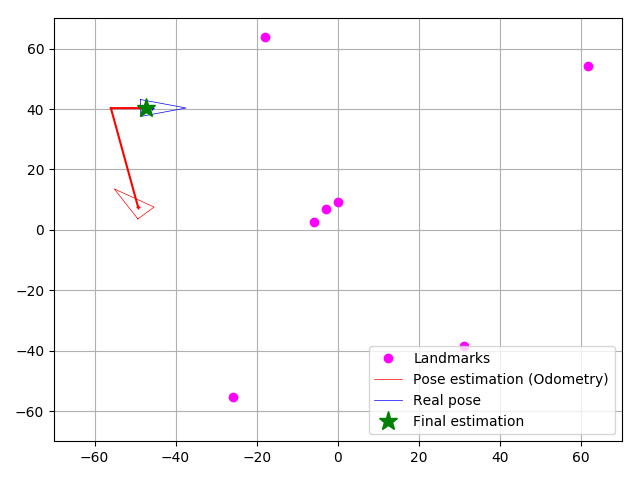
\includegraphics{images/fig5-1-1.png}
\end{figure}

    \begin{tcolorbox}[breakable, size=fbox, boxrule=1pt, pad at break*=1mm,colback=cellbackground, colframe=cellborder]
\prompt{In}{incolor}{12}{\boxspacing}
\begin{Verbatim}[commandchars=\\\{\}]
\PY{k}{def} \PY{n+nf}{main}\PY{p}{(}\PY{n}{nLandmarks}\PY{o}{=}\PY{l+m+mi}{7}\PY{p}{,} \PY{n}{env\PYZus{}size}\PY{o}{=}\PY{l+m+mi}{140}\PY{p}{)}\PY{p}{:}
    \PY{c+c1}{\PYZsh{} MATPLOTLIB}
    \PY{n}{fig}\PY{p}{,} \PY{n}{ax} \PY{o}{=} \PY{n}{plt}\PY{o}{.}\PY{n}{subplots}\PY{p}{(}\PY{p}{)}
    \PY{n}{plt}\PY{o}{.}\PY{n}{xlim}\PY{p}{(}\PY{p}{[}\PY{o}{\PYZhy{}}\PY{l+m+mi}{90}\PY{p}{,} \PY{l+m+mi}{90}\PY{p}{]}\PY{p}{)}
    \PY{n}{plt}\PY{o}{.}\PY{n}{ylim}\PY{p}{(}\PY{p}{[}\PY{o}{\PYZhy{}}\PY{l+m+mi}{90}\PY{p}{,} \PY{l+m+mi}{90}\PY{p}{]}\PY{p}{)}
    \PY{n}{plt}\PY{o}{.}\PY{n}{grid}\PY{p}{(}\PY{p}{)}
    \PY{n}{plt}\PY{o}{.}\PY{n}{ion}\PY{p}{(}\PY{p}{)}
    \PY{n}{plt}\PY{o}{.}\PY{n}{tight\PYZus{}layout}\PY{p}{(}\PY{p}{)}

    \PY{n}{fig}\PY{o}{.}\PY{n}{canvas}\PY{o}{.}\PY{n}{draw}\PY{p}{(}\PY{p}{)}
    
    \PY{c+c1}{\PYZsh{} VARIABLES}
    \PY{n}{num\PYZus{}landmarks} \PY{o}{=} \PY{l+m+mi}{7} \PY{c+c1}{\PYZsh{} number of landmarks in the environment}
    \PY{n}{env\PYZus{}size} \PY{o}{=} \PY{l+m+mi}{140} \PY{c+c1}{\PYZsh{} A square environment with x=[\PYZhy{}env\PYZus{}size/2,env\PYZus{}size/2] and y=[\PYZhy{}env\PYZus{}size/2,env\PYZus{}size/2]}
       
    \PY{c+c1}{\PYZsh{} MAP CREATION AND VISUALIZATION}
    \PY{n}{w\PYZus{}map} \PY{o}{=} \PY{n}{env\PYZus{}size}\PY{o}{*}\PY{n}{scipy}\PY{o}{.}\PY{n}{rand}\PY{p}{(}\PY{l+m+mi}{2}\PY{p}{,} \PY{n}{num\PYZus{}landmarks}\PY{p}{)} \PY{o}{\PYZhy{}} \PY{n}{env\PYZus{}size}\PY{o}{/}\PY{l+m+mi}{2} \PY{c+c1}{\PYZsh{} randomly place the landmarks in the map}
    \PY{n}{ax}\PY{o}{.}\PY{n}{plot}\PY{p}{(}\PY{n}{w\PYZus{}map}\PY{p}{[}\PY{l+m+mi}{0}\PY{p}{,} \PY{p}{:}\PY{p}{]}\PY{p}{,} \PY{n}{w\PYZus{}map}\PY{p}{[}\PY{l+m+mi}{1}\PY{p}{,} \PY{p}{:}\PY{p}{]}\PY{p}{,} \PY{l+s+s1}{\PYZsq{}}\PY{l+s+s1}{o}\PY{l+s+s1}{\PYZsq{}}\PY{p}{,} \PY{n}{color}\PY{o}{=}\PY{l+s+s1}{\PYZsq{}}\PY{l+s+s1}{magenta}\PY{l+s+s1}{\PYZsq{}}\PY{p}{,} \PY{n}{label}\PY{o}{=}\PY{l+s+s2}{\PYZdq{}}\PY{l+s+s2}{Landmarks}\PY{l+s+s2}{\PYZdq{}}\PY{p}{)}
    
    \PY{c+c1}{\PYZsh{} ROBOT POSE AND SENSOR INITIALIZATION }
    \PY{n}{desv\PYZus{}d} \PY{o}{=} \PY{l+m+mf}{0.5} \PY{c+c1}{\PYZsh{} standard deviation (noise) of the range measurement}
    \PY{n}{cov} \PY{o}{=} \PY{n}{np}\PY{o}{.}\PY{n}{diag}\PY{p}{(}\PY{p}{[}\PY{l+m+mi}{25}\PY{p}{,} \PY{l+m+mi}{30}\PY{p}{,} \PY{n}{np}\PY{o}{.}\PY{n}{pi}\PY{o}{*}\PY{l+m+mi}{180}\PY{p}{]}\PY{p}{)}\PY{o}{*}\PY{o}{*}\PY{l+m+mi}{2} \PY{c+c1}{\PYZsh{} covariance of the motion (odometry)}
    \PY{n}{xStart} \PY{o}{=} \PY{n}{np}\PY{o}{.}\PY{n}{vstack}\PY{p}{(}\PY{n}{plt}\PY{o}{.}\PY{n}{ginput}\PY{p}{(}\PY{l+m+mi}{1}\PY{p}{)}\PY{p}{)}\PY{o}{.}\PY{n}{T} \PY{c+c1}{\PYZsh{} get the robot starting point from the user}
    \PY{n}{robot\PYZus{}pose}\PY{o}{=}\PY{n}{np}\PY{o}{.}\PY{n}{vstack}\PY{p}{(}\PY{p}{[}\PY{n}{xStart}\PY{p}{,} \PY{l+m+mi}{0}\PY{p}{]}\PY{p}{)} \PY{c+c1}{\PYZsh{} robot\PYZus{}pose}
    
    \PY{n}{R1} \PY{o}{=} \PY{n}{Robot}\PY{p}{(}\PY{n}{robot\PYZus{}pose}\PY{p}{,} \PY{n}{cov}\PY{p}{,} \PY{n}{desv\PYZus{}d}\PY{p}{)}
    \PY{n}{R1}\PY{o}{.}\PY{n}{plot}\PY{p}{(}\PY{n}{fig}\PY{p}{,} \PY{n}{ax}\PY{p}{)}

    \PY{c+c1}{\PYZsh{} MAIN}
    \PY{n}{z} \PY{o}{=} \PY{n}{distance}\PY{p}{(}\PY{n}{R1}\PY{o}{.}\PY{n}{true\PYZus{}pose}\PY{p}{,} \PY{n}{w\PYZus{}map}\PY{p}{,} \PY{n}{cov\PYZus{}d}\PY{o}{=}\PY{n}{R1}\PY{o}{.}\PY{n}{var\PYZus{}d}\PY{p}{)} \PY{c+c1}{\PYZsh{} take (noisy) measurements to the landmarks}
    \PY{n}{LeastSquaresLocalization}\PY{p}{(}\PY{n}{R1}\PY{p}{,} \PY{n}{w\PYZus{}map}\PY{p}{,} \PY{n}{z}\PY{p}{)} \PY{c+c1}{\PYZsh{} LS Positioning!}
    
    \PY{c+c1}{\PYZsh{} PLOTTING RESULTS}
    \PY{n}{plt}\PY{o}{.}\PY{n}{legend}\PY{p}{(}\PY{p}{)}
    \PY{n}{fig}\PY{o}{.}\PY{n}{canvas}\PY{o}{.}\PY{n}{draw}\PY{p}{(}\PY{p}{)}

\PY{c+c1}{\PYZsh{} RUN    }
\PY{n}{main}\PY{p}{(}\PY{p}{)}
\end{Verbatim}
\end{tcolorbox}

\begin{figure}
\centering
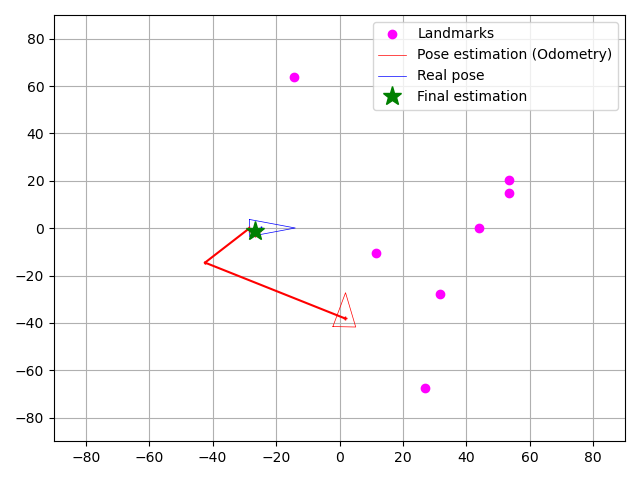
\includegraphics{images/lastOutput_1.png}
\end{figure}

    \begin{Verbatim}[commandchars=\\\{\}]
Iteration :0
  delta :   [ 44.0057992  -23.49943717]
  residual: 74.36026143865935
Iteration :1
  delta :   [-13.8067084  -14.31290261]
  residual: 41.801658718863955
Iteration :2
  delta :   [-1.82674997  1.22172869]
  residual: 15.799693618983511
Iteration :3
  delta :   [-0.06327266 -0.11998843]
  residual: 15.48848431213921
Iteration :4
  delta :   [-0.00179557  0.00502551]
  residual: 15.492276132655476
Iteration :5
  delta :   [-5.39681359e-05 -2.99526073e-04]
  residual: 15.492877592728162
    \end{Verbatim}

    \hypertarget{thinking-about-it-1}{%
\subsubsection{Thinking about it (1)}\label{thinking-about-it-1}}

Having completed this notebook above, you will be able to \textbf{answer
the following questions}:

\begin{itemize}
\item
  What are the dimensions of the error residuals? Does them depend on
  the number of observations?

  3x1. No, its depend on the number of elements in pose (in our case 3;
  {[}x,y,angle{]})
\item
  Why is Weighted LS obtaining better results than LS?

  Because now we are weighing the different distances to landmarks
  having in count the uncertainty of sensors, making the measurements of
  the robot to locate itself more precise.
\item
  Which is the minimum number of landmarks needed for localizing the
  robot? Why?

  In our case 3. Because we need as many landmarks as elements make up
  our pose, in orer to solve the system of equations. In case we did not
  have the minimun number of landmarks, there would be infinite
  solutions
\item
  Play with different ``qualities'' of the range sensor. Could you find
  a value for its variance so the LS method fails?

  Yes. It fails when the standard desviation of the sensors is 0.
\item
  Play also with different values for the odometry uncertainty. What
  does this affect?

  This affects where the robot thinks it is. The higher the values, the
  greater the probability that the robot is further from the real pose. 
  The lower the values, the closer it is to the real pose.
\end{itemize}


    % Add a bibliography block to the postdoc
    
    
    
\end{document}
